\section{am::lambda::binder1$<$ R, P1, A1 $>$ Struct Template Reference}
\label{structam_1_1lambda_1_1binder1}\index{am::lambda::binder1@{am::lambda::binder1}}
{\tt \#include $<$lambda.hpp$>$}

Inherits {\bf am::lambda::detail::lambda\_\-op\_\-tag}.

Inheritance diagram for am::lambda::binder1$<$ R, P1, A1 $>$:\begin{figure}[H]
\begin{center}
\leavevmode

\includegraphics[width=108pt]{structam_1_1lambda_1_1binder1__inherit__graph}
\end{center}
\end{figure}
Collaboration diagram for am::lambda::binder1$<$ R, P1, A1 $>$:\begin{figure}[H]
\begin{center}
\leavevmode
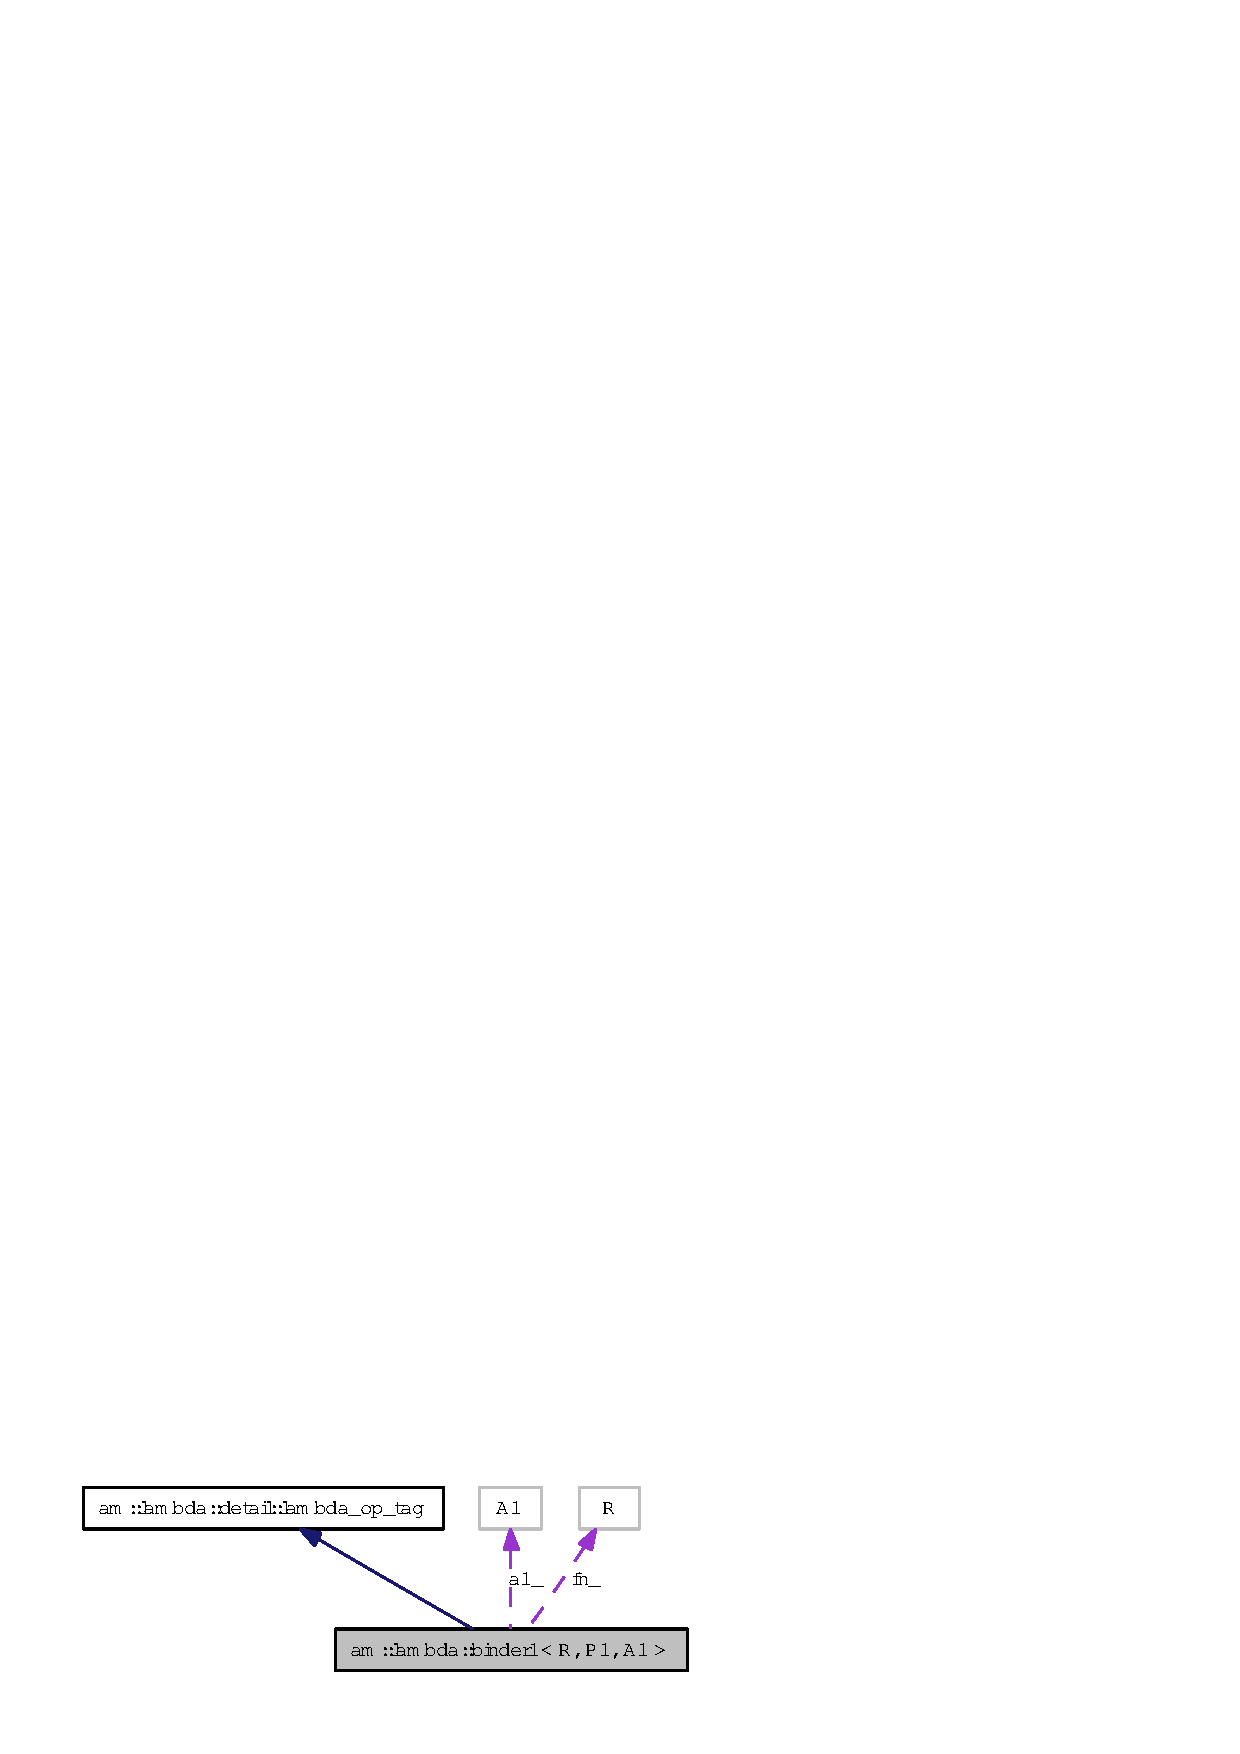
\includegraphics[width=166pt]{structam_1_1lambda_1_1binder1__coll__graph}
\end{center}
\end{figure}
\subsection*{Public Types}
\begin{CompactItemize}
\item 
typedef detail::binder\_\-impl$<$ R $>$::result\_\-type \textbf{result\_\-type}\label{structam_1_1lambda_1_1binder1_9ca2fec190c6c2d883b66b4d3522c95b}

\end{CompactItemize}
\subsection*{Public Member Functions}
\begin{CompactItemize}
\item 
\textbf{binder1} (R($\ast$fn)(P1), A1 a1)\label{structam_1_1lambda_1_1binder1_c2108aaef80abd01a31bce2a0e38c6a3}

\item 
template$<$class T1, class T2, class T3$>$ result\_\-type \textbf{operator()} (T1 t1, T2 t2, T3 t3) const \label{structam_1_1lambda_1_1binder1_480bdebf86834c60e81bd98e82ae1eb9}

\item 
template$<$class T1, class T2$>$ result\_\-type \textbf{operator()} (T1 t1, T2 t2) const\label{structam_1_1lambda_1_1binder1_e3b600bffd6e5564189362b838a5e341}

\item 
template$<$class T1$>$ result\_\-type \textbf{operator()} (T1 t1) const \label{structam_1_1lambda_1_1binder1_2f055604a17c90630328a6fe236387d4}

\item 
result\_\-type \textbf{operator()} () const\label{structam_1_1lambda_1_1binder1_1238e7e2aec16f220493f12e385c5808}

\end{CompactItemize}
\subsection*{Public Attributes}
\begin{CompactItemize}
\item 
R($\ast$ \textbf{fn\_\-} )(P1)\label{structam_1_1lambda_1_1binder1_54e5220f72cf932262c966ed61ba42fb}

\item 
A1 \textbf{a1\_\-}\label{structam_1_1lambda_1_1binder1_e83629cd1c47a8a452918e8b6bc12845}

\end{CompactItemize}


\subsection{Detailed Description}
\subsubsection*{template$<$typename R, typename P1, typename A1$>$ struct am::lambda::binder1$<$ R, P1, A1 $>$}

Binder for the free function which takes one argument. 



The documentation for this struct was generated from the following file:\begin{CompactItemize}
\item 
{\bf lambda.hpp}\end{CompactItemize}
